\documentclass{ase}

\usepackage{graphicx}
\usepackage{acronym}
\usepackage{listings}
\usepackage{vdmlisting}
\usepackage{appendix}
\usepackage{xspace}

\acrodef{ast}[AST]{Abstract Syntax Tree}
\acrodef{vdm}[VDM]{Vienna Development Method}
\acrodef{jml}[JML]{Java Modeling Language}
\acrodef{dbc}[DbC]{Design-by-Contract}
\acrodef{atm}[ATM]{Automated Teller Machine}
\acrodef{pvs}[PVS]{the Prototype Verification System}
\acrodef{uml}[UML]{the Unified Modeling Language}
\acrodef{ir}[IR]{Intermediate Representation}

\newcommand{\vsl}{VDM-SL\xspace}

\lstset{
    basicstyle=\footnotesize\ttfamily,
    frame=single, 
    breaklines=true,
    tabsize=2, 
    linewidth=\columnwidth,
    showstringspaces=false, 
    captionpos=b,
    frameround=, 
    aboveskip=5mm,
    belowskip=5mm,
    framexleftmargin=0mm, 
    framexrightmargin=0mm,
    escapeinside={(*@}{@*)},
%    numbers=left,               
%    numbersep=10pt,                   
%    numberstyle=\small,
}


\title{Automated translation of VDM-SL to JML annotated Java}
\subtitle{Technical Report}
\author{Peter W. V. Tran-J\o{}rgensen}

\reportid{TR-XX}
\frontlogo{figs/logo}
%\makenomenclature
\begin{document}

\maketitle
\frontmatter
\asetableofcontents

\mainmatter


\chapter{Introduction}

A model specified using the \ac{vdm} can be validated against its
contract-based elements (e.g.\ pre and postconditions and invariants)
in order to ensure that the system behaves as intended. One way to
validate the model against its contracts is by animation using
Overture's \ac{vdm} interpreter.

When sufficient insight into the system under development has been
obtained during the formal analysis, development proceeds to the
implementation phase, where the system is realised. One way to realise
a \ac{vdm} model is by implementing it in a programming language, for
example, using code generation. However, since no guarantees are made
about the correctness of the generated code, other measures must be
taken to increase the confidence in the correctness of the generated
code.

To support this approach, Overture enables fully automated translation
of \vsl's contract-based elements (pre- and postconditions, and
invariants) and type constraints to \ac{jml} annotations. The \ac{jml}
generator is developed as an extension of Overture's \ac{vdm}-to-Java
code generator and produces \ac{jml} annotated Java programs. In this
way \ac{jml} tools can be used to validate the generated Java code
against the \emph{intended} system behaviour, described using
\ac{jml}. This work-flow is illustrated in
\cref{fig:vdm2jml-overview}.

\begin{figure}[!ht]
  \centering
  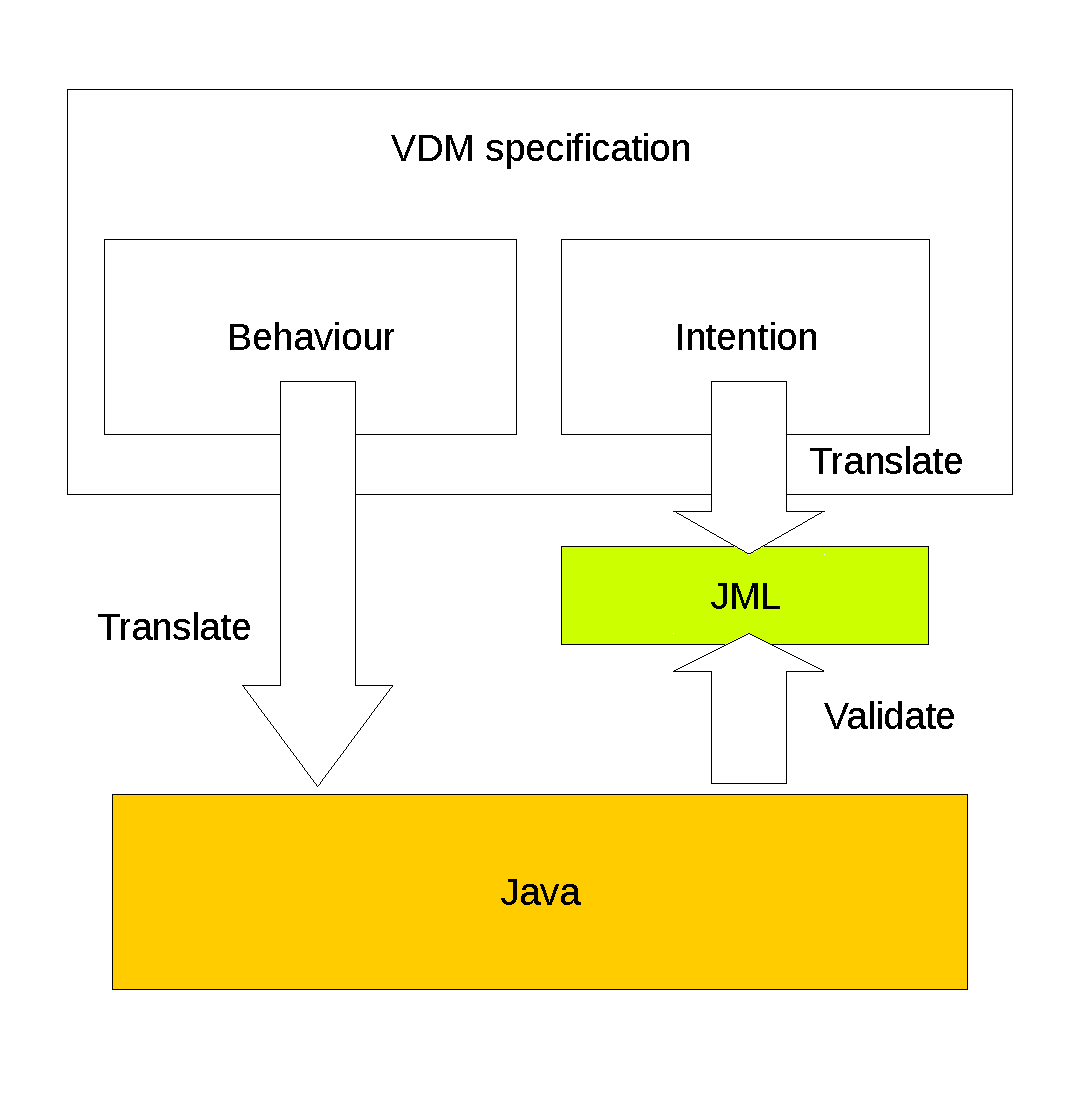
\includegraphics[width=0.6\linewidth]{figs/vdm2jml}
  \caption {Overview of the \ac{vdm}-to-JML translation.}
  \label{fig:vdm2jml-overview}
\end{figure}

\subsection{Background}

The translation is defined as a set of rules that are implemented as
an extension of Overture \ac{vdm}-to-Java code
generator~\cite{Jorgensen&14a} to make the approach fully automated.

\subsection{Prerequisites}

\begin{itemize}
\item Mention OpenJML
\item Mention rules and VDM-to-JML paper
\item Mention Overture
\end{itemize}

%%% Local Variables:
%%% mode: latex
%%% TeX-master: "../vdm2jml-tr"
%%% End:


\begin{appendices}
  
\chapter{\ac{atm} Example}

This appendix includes the complete version of the \vsl \ac{atm}
example used to demonstrate the \ac{jml} translation presented
in~\cite{Jorgensen&16a} as well as this technical report.

\lstinputlisting[language=VDM_SL]{listings/ATM.vdmsl}

%%% Local Variables:
%%% mode: latex
%%% TeX-master: "../vdm2jml-tr"
%%% End:

\end{appendices}

%\addcontentsline{toc}{chapter}{Bibliography}
\bibliographystyle{splncs03}
\bibliography{refs}

\end{document}
